\documentclass[tikz,margin=2mm]{standalone}
\usepackage{tikz}
\usetikzlibrary{shapes.geometric}
\pagecolor{white}
\begin{document}
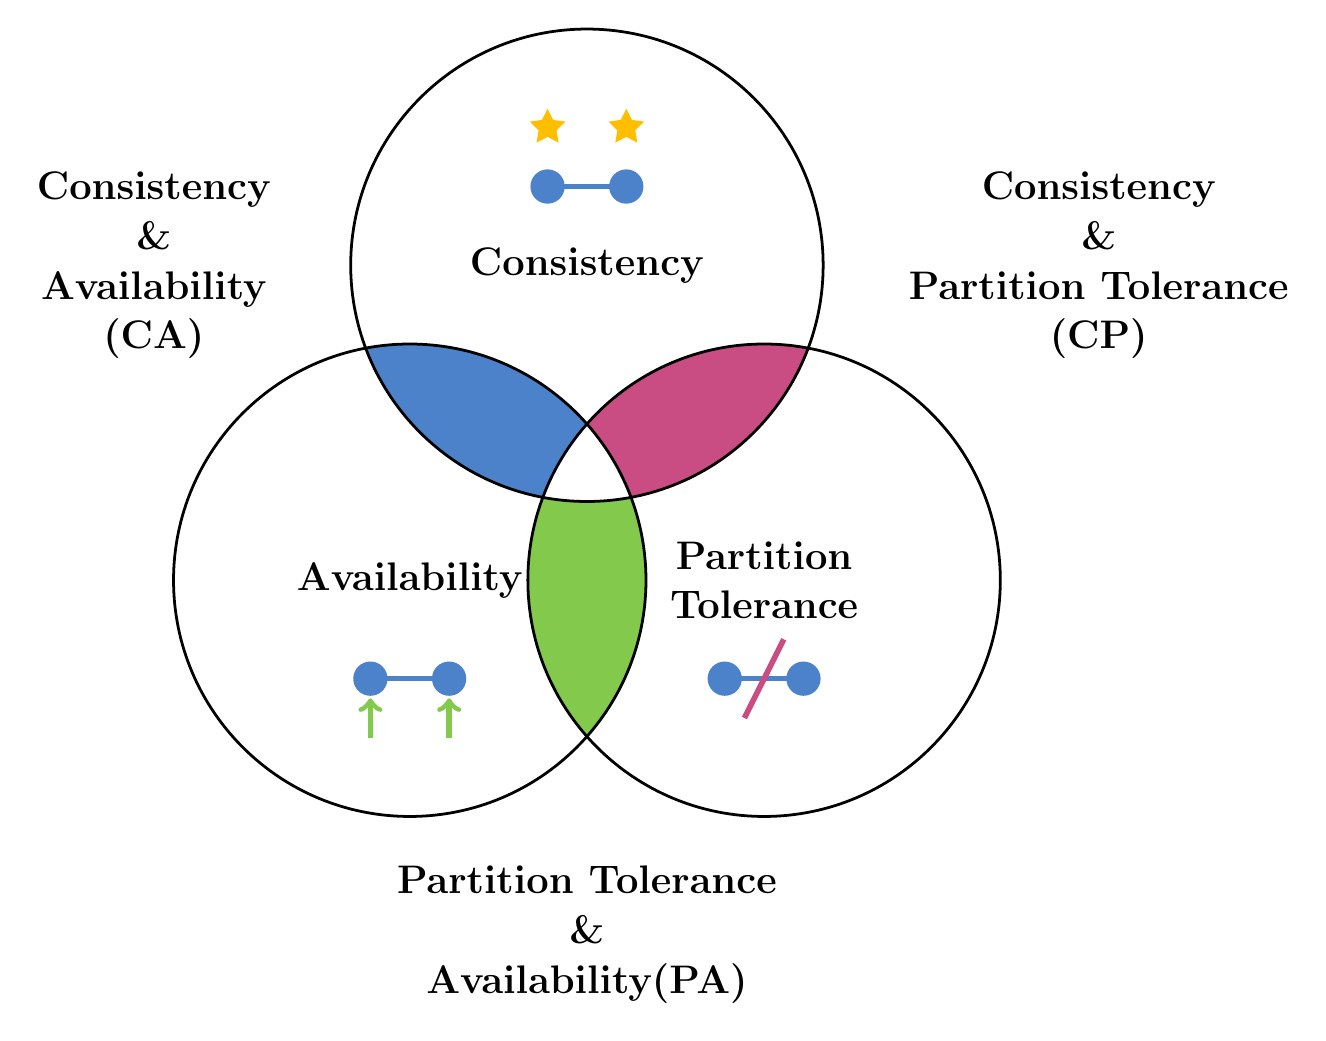
\begin{tikzpicture}[line width=1pt, x=10mm,y=10mm]
  \coordinate (A) at (08.25,5);
  \coordinate (B) at (12.75,5);
  \coordinate (C) at (10.5,9);

  \fill[white, draw=none] (A) circle (3);
  \fill[white, draw=none] (B) circle (3);
  \fill[white, draw=none] (C) circle (3);
  
  \begin{scope}
    \clip (A) circle (3);
    \fill[green!70!red!70, draw=none] (B) circle (3);
  \end{scope}
  
  \begin{scope}
    \clip (B) circle (3);
    \fill[red!70!blue!70, draw=none] (C) circle (3);
  \end{scope}

  \begin{scope}
    \clip (C) circle (3);
    \fill[blue!70!green!70, draw=none] (A) circle (3);
  \end{scope}

  \begin{scope}
    \clip (A) circle (3);
    \clip (B) circle (3);
    \fill[white, draw=none] (C) circle (3);
  \end{scope}

  \draw[line width=1pt] (A) circle (3);
  \draw[line width=1pt] (B) circle (3);
  \draw[line width=1pt] (C) circle (3);

  \node at (A) [align=center, font=\bfseries\Large] {Availability};
  \node at (B) [align=center, font=\bfseries\Large] {Partition\\Tolerance};
  \node at (C) [align=center, font=\bfseries\Large] {Consistency};

  \node at (5,9) [align=center, font=\bfseries\Large] {Consistency\\\&\\Availability\\(CA)};
  \node at (17,9) [align=center, font=\bfseries\Large] {Consistency\\\&\\Partition Tolerance\\(CP)};
  \node at (10.5,0.5) [align=center, font=\bfseries\Large] {Partition Tolerance\\\&\\Availability(PA)};

  \draw[color=blue!70!green!70, line width=2] (10,10) -- (11,10);
  \draw[color=blue!70!green!70, fill=blue!70!green!70](10,10) circle (0.2);
  \draw[color=blue!70!green!70, fill=blue!70!green!70](11,10) circle (0.2);

  \draw[color=blue!70!green!70, line width=2] (7.75,3.75) -- (8.75,3.75);
  \draw[color=blue!70!green!70, fill=blue!70!green!70](7.75,3.75) circle (0.2);
  \draw[color=blue!70!green!70, fill=blue!70!green!70](8.75,3.75) circle (0.2);

  \draw[color=blue!70!green!70, line width=2] (12.25,3.75) -- (13.25,3.75);
  \draw[color=blue!70!green!70, fill=blue!70!green!70](12.25,3.75) circle (0.2);
  \draw[color=blue!70!green!70, fill=blue!70!green!70](13.25,3.75) circle (0.2);

  \node[star, star points=5, star point ratio=2,
    draw=orange!50!yellow, fill=orange!50!yellow, inner sep=2pt] at (10,10.75) {};
  \node[star, star points=5, star point ratio=2,
    draw=orange!50!yellow, fill=orange!50!yellow, inner sep=2pt] at (11,10.75) {};

  \draw[color=red!70!blue!70, line width=2] (12.5,3.25) -- (13.0,4.25);

  \draw[->, color=green!70!red!70, line width=2pt] (7.75,3) -- (7.75,3.5);
  \draw[->, color=green!70!red!70, line width=2pt] (8.75,3) -- (8.75,3.5);
\end{tikzpicture}
\end{document}
